\subsection{Current Solution}
\label{description:solution}

Currently, there exists the functionality in Tomboy to create bullet lists and different Tomboy notes with links inbetween them.

There existed a project (also realized as an Addin) for task management, called \textit{Tasks}, maintained by %TODO who?
for quite some time. However, this was removed in Version 0.9.3 %TODO sure?
of Tomboy, because it did not meet the design constraints. It was a totally separate task management UI in Tomboy that was not integrated into the existing note structure at all. The maintainer, ???, abandoned then the code of that and created a new program called \textit{Tasque} that was now entirely concentrating on task management, leaving Tomboy without any such capability again.

Later, a new Addin was initiated, but never finished by Sandy Armstring. This project, called \textit{TaskLists} is still in a very early phase, has not yet much functionality and still contains many bugs. Also, at the moment nobody is working on it.

In summary, the \textbf{basic problem} until now was that only a too simple solution (bullet lists) was available, and the solution that was created at the beginning was too different from Tomboy to be really integrated. The Tasks Addin had additional windows and things like that within Tomboy that made it look more like a separate application besides Tomboy instead of an Addin, what is also the reason it was outsourced to a separate product.

Our goal is to finish such a project up to a stable and working solution (in terms of \textit{bug-freeness} and \textit{usability}) that is fully integrated into Tomboy and easy and simple to use, such that it could finally be included into the official Tomboy project.

\subsection{Product Perspective}
\label{description:perspective}
  The project TaskList will be part of the Tomboy project. There will be three main interfaces:

  \begin{itemize}
    \item The first one is the obvious user interface that the user sees within Tomboy.
    \item Then, the representation of data will be done via Tomboy note files. That means, persistent storage of the Tasks must be accomplished as xml files within the Tomboy notes file structure.
    \item Also, saving and retrieving data (for example, import and export of notes from/to other note taking applications) will be done using XML files.
  \end{itemize}

  Also, for an overwie of the integration of TaskList within the Tomboy/GTK/Mono context, see figure \ref{perspective}.

  \begin{figure}[h]
    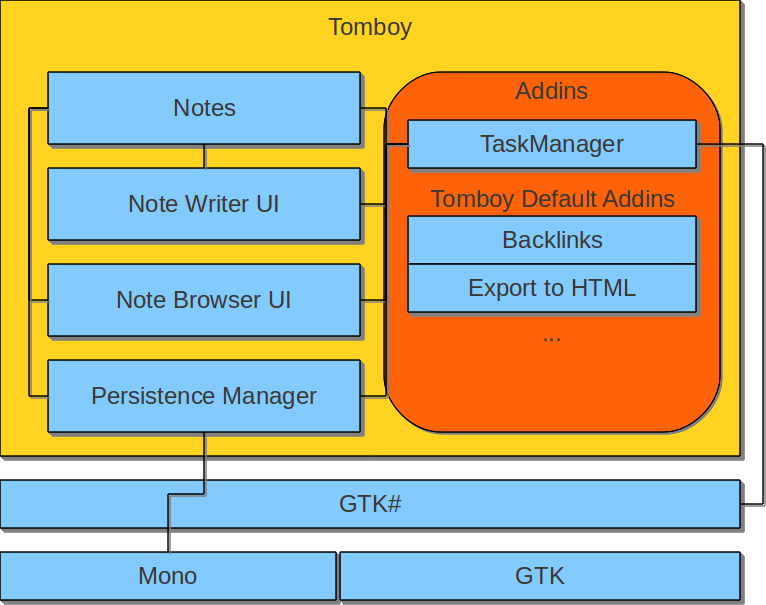
\includegraphics[width=\textwidth]{graphics/product_perspective_diagram.png}
    \caption{TaskList Product Perspective}
    \label{perspective}
  \end{figure}


\subsection{Product Functions}
\label{description:functions}

  \subsubsection*{Supported Functions}
  \label{description:functions:supported}

    \begin{itemize}
      \item Provides Task management capabilities for Tomboy
      \item Supports multiple Tasks and TaskLists as well as Subtasks
      \item Supports priorities and due dates
      \item Allows to create dependencies between tasks
      \item Allows easy management of TaskLists and Tasks
      \item Allows to import export TaskLists
    \end{itemize}

    \subsubsection*{Unsupported Functions}
      \label{description:functions:unsupported}
      \begin{itemize}
        \item Does not have additional GUI windows or external tools within or outside of Tomboy. (SEE ?) %TODO reference
        \item Does not support synchronisation with external tools or clients except for manual export / import.
      \end{itemize}

\subsection{User Characteristics}
\label{description:usercharacteristics}

  \begin{itemize}
    \item[Casual user] The casual user will create simple task lists. He may or may not know very vell the functionality of Tomboy. Still, he should be able to create simple TaskLists where he can cross out individual elements easily.

    \item [Advanced user] The advanced user knows and uses Tomboy already quite well. He should be able without too much effort to add arguments such as due dates and priorities to his task lists, create hierarichies of tasks and may his lists to other tools, e.g. \textit{Evolution}.
  \end{itemize}


\subsection{Constraints}
\label{description:constraints}
The Addin itself should obey all criterias (standards and guidelines) imposed by the GNOME and Tomboy projects (SEE ?). %TODO

Besides the coding guidelines this includes mainly design aspects, such as simplicity and easyness of use, and full integration into Tomboy (see also \ref{?}).


\subsection{Assumptions and Dependencies}
\label{description:assumptions}

